\documentclass[12pt]{article}
\usepackage[margin=1in]{geometry} 
\usepackage{amsmath}
\usepackage{amssymb}
\usepackage{siunitx}
\usepackage{float}
\usepackage{tikz}
\def\checkmark{\tikz\fill[scale=0.4](0,.35) -- (.25,0) -- (1,.7) -- (.25,.15) -- cycle;} 
\usepackage{url}
\usepackage[siunitx,american,RPvoltages]{circuitikz}
\ctikzset{capacitors/scale=0.7}
\ctikzset{diodes/scale=0.7}
\usepackage{tabularx}
\newcolumntype{C}{>{\centering\arraybackslash}X}
\renewcommand\tabularxcolumn[1]{m{#1}}% for vertical centering text in X column
\usepackage{tabu}
\usepackage[spanish,es-tabla,activeacute]{babel}
\usepackage{babelbib}
\usepackage{booktabs}
\usepackage{pgfplots}
\usepackage{hyperref}
\hypersetup{colorlinks = true,
            linkcolor = black,
            urlcolor  = blue,
            citecolor = blue,
            anchorcolor = blue}
\usepgfplotslibrary{units, fillbetween} 
\pgfplotsset{compat=1.16}
\usepackage{bm}
\usetikzlibrary{arrows, arrows.meta, shapes, 3d, perspective, positioning,mindmap,trees,backgrounds}
\renewcommand{\sin}{\sen} %change from sin to sen
\usepackage{bohr}
\setbohr{distribution-method = quantum,insert-missing = true}
\usepackage{elements}
\usepackage{verbatim}
\usepackage[edges]{forest}
\usepackage{etoolbox}
\usepackage{schemata}
\usepackage{appendix}
\usepackage{listings}

\definecolor{color_mate}{RGB}{255,255,128}
\definecolor{color_plas}{RGB}{255,128,255}
\definecolor{color_text}{RGB}{128,255,255}
\definecolor{color_petr}{RGB}{255,192,192}
\definecolor{color_made}{RGB}{192,255,192}
\definecolor{color_meta}{RGB}{192,192,255}
\newcommand\diagram[2]{\schema{\schemabox{#1}}{\schemabox{#2}}}

\definecolor{codegreen}{rgb}{0,0.6,0}
\definecolor{codegray}{rgb}{0.5,0.5,0.5}
\definecolor{codepurple}{rgb}{0.58,0,0.82}
\definecolor{backcolour}{rgb}{0.95,0.95,0.92}

\lstdefinestyle{mystyle}{
    backgroundcolor=\color{backcolour},   
    commentstyle=\color{codegreen},
    keywordstyle=\color{magenta},
    numberstyle=\tiny\color{codegray},
    stringstyle=\color{codepurple},
    basicstyle=\ttfamily\footnotesize,
    breakatwhitespace=false,         
    breaklines=true,                 
    captionpos=b,                    
    keepspaces=true,                 
    numbers=left,                    
    numbersep=5pt,                  
    showspaces=false,                
    showstringspaces=false,
    showtabs=false,                  
    tabsize=2
}

\lstset{style=mystyle}
\usepackage{lastpage}
\usepackage{fancyhdr}
\usepackage{enumitem}
\usepackage{csvsimple,booktabs}
\pagestyle{fancy}
\setlength{\headheight}{42pt}

 
\begin{document}
\lhead{Ingeniería Física \\ Escuela de Física \\ Tecnológico de Costa Rica} 
\rhead{Instrumentación I \\ Tarea \#1  \\ Entrega: Semana 4} 
\cfoot{\thepage\ de \pageref{LastPage}}
\setlength{\parindent}{0em}

A partir del diagrama incluido en la Figura \ref{t1f1} y usando el estándar \href{http://integrated.cc/cse/Instrumentation_Symbols_and_Identification.pdf}{ANSI/ISA-5.1-2009}.
Realice los siguiente:
\begin{enumerate}
    \item Para cada uno de los elementos de la figura que estan incluidos en el estándar incluya*: 
    \begin{enumerate}
        \item Símbolo
        \item Breve descripción
        \item Variable a medir o controlar en caso de instrumentos de medición o control
        \item Tabla de la norma donde aparece. Por ejemplo: Tabla 5.2.4        
    \end{enumerate}
    \item Indique al menos dos mejoras que usted incluiría en el digrama según el estándar
\end{enumerate}
\begin{figure}[H]
    \centering
    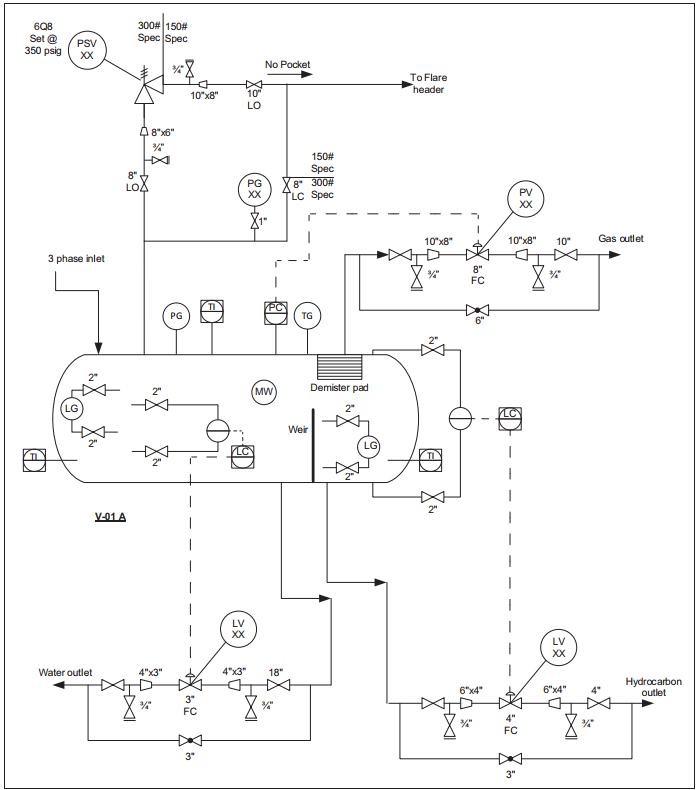
\includegraphics[width = 0.6\linewidth]{fig/diagrama1.png}
    \caption{Separador de tres fases}
    \label{t1f1}
\end{figure}
* Si algún elemento aparece varias veces se debe incluir una sola vez
\end{document}